\documentclass{article}
\usepackage{graphicx} % Required for inserting images
\usepackage{hyperref}
\usepackage{float}

\title{CS695 Assignment4}
\author{Josyula Venkata Aditya - 210050075 \\ Ananth Krishna Kidambi - 210051002}

\begin{document}

\maketitle

\section{Introduction}
Our assignment is based on implementing FaaS(Function as a Service) using kubernetes. It is a fairly simple version of FaaS and we aim to provide the following features.
\begin{itemize}
    \item Registration of endpoints
    \item Isolation of namespaces among organizations
    \item Registration of triggers for endpoints through a docker registry
    \item Autoscaling pods based on load 
    \item Removal of inactive pods 
\end{itemize}
As we go along, we will look into more of these features. Note that we are not supporting triggering function DAGs as of now, triggers can only be standalone functions without side effects, but it is possible to extend support to side effects being restricted to disk changes by using a NFS instead of a disk on each node.

\section{Setup}

We have setup our cluster using 3 virtual machines running on a server, one of them functioning as the control plane and the other two functioning as the worker nodes. The specs of the virtual machines are as follows:
\begin{itemize}
    \item RAM: 4 GB (excluding swap)
    \item 4 CPU cores
    \item Operating System: Ubuntu-22.04 
\end{itemize}
There is no router between the virtual machines, all of them lie on the same LAN. If you would want to reproduce the results, it is highly suggested to use physical machines/virtual machines that lie on the same LAN without any router in between them since we have faced problems with setting up the CNI (Container Network Interface), calico in our case, in such a setup. The versions of Kubernetes and calico are as follows:
\begin{itemize}
    \item Kubeadm version: 1.30.0
    \item Kubelet version: 1.30.0
    \item Kubectl version: 1.30.0
    \item Calico: \href{https://raw.githubusercontent.com/projectcalico/calico/v3.27.3/manifests/calico-typha.yaml}{Link to the yaml file we used}
\end{itemize}
The node running the control plane is the main server for handling user requests in our FaaS implementation. We have not made its IP  address externally available hence the FaaS service is accessible only within the private area network.

\section{User API}
A python process on the control plane node runs a multithreaded \texttt{Flask} server that first accepts requests from the user and then deploys containers appropriately to service the user requests. Once the request is serviced by a container, the output is returned back to the user from the \texttt{Flask} server. The format of our FaaS endpoints is \texttt{http://<IP address>:8887/<organization>/<endpoint name>}. Here, \texttt{IP address} is the IP address of the node running the \texttt{Flask} server, which is the control plane in our case.
\subsection{Registering endpoints}
First, we would need a way to install/manage the dependencies of the trigger function when the control plane wishes to deploy it. A docker image is a straightforward solution for such tasks and we have adopted this approach in our solution as well. An \texttt{src} folder with all the files required to run the function has to be provided, from which an image will be generated and pushed to our private docker registry running on another computer in the same private network. Note that we did not choose DockerHub for this purpose because there is a limit on the number of image pulls an IP address can make in a day, and this interferes with the process of testing our implementation. Once the image is pushed, a request has to be made at a special endpoint on the server \texttt{http://<IP-address>:8887/add\_endpoint}. This request expects a json payload with the following attributes:
\begin{itemize}
    \item \texttt{org} : This is the name of the organization. If this is a new organization, a new namespace is created for this organization and all the entities related to the organization will be put in this namespace
    \item \texttt{endpoint} : This is the endpoint that the organization wants to register with a FaaS trigger function.
    \item \texttt{image} : This is the name of the image in the docker registry which must be used to execute the trigger function
    \item \texttt{replicas} : This indicates the number of pod replicas to be run for this particular endpoint.
\end{itemize}

\section{Implementation}
We use \texttt{kubernetes} as the container orchestrator and \texttt{docker} as the container manager. In addition, a third-party CNI has to be installed to facilitate networking between the pods. After having gone through multiple failed attempts, we would suggest that if you are using \texttt{calico} for CNI, then connect the nodes using a LAN with no router in between, this makes sure that all the nodes are on the same subnet, and hence BGP used by \texttt{calico} wouldn't cause issues. \texttt{Flannel} is another choice for CNI. Also, \texttt{swap} must be disabled on the nodes and control plane for kubernetes to work correctly. We also use a private docker registry instead of DockerHub for reasons mentioned in a previous section. Also, it is suggested to have at least 4 GB of RAM and a large enough disk to avoid memory pressure and disk pressure while running the cluster. \\
We use python's \texttt{Flask} API to implement the central server that would first receive all the user requests. The server also uses kubernetes' python API to facilitate deployment from within the server process. We also maintain a database storing the information about the endpoints and the organizations.
\begin{itemize}
    \item Table \texttt{organization} just stores the names of organizations
    \item Table \texttt{endpoints} stores the following:
    \begin{itemize}
        \item name of the organization
        \item name of the endpoint
        \item IP address of the ClusterIP service
        \item the image to use for deploying a container when trigger is given
        \item The number of replicas of pods to use for this endpoint trigger.
    \end{itemize}
\end{itemize}
Whenever an endpoint is registered, appropriate modifications are made to the tables. In addition to the files provided in the \texttt{src} folder, we add an additional file called \texttt{.interface.py} in the docker image. This runs a \texttt{Flask} server inside the container to receive the forwarded request from the central server and then calls the trigger function on the received request. It then sends the return value back to the central server in the form of a request which is then forwarded to the user. 

To streamline the process of deploying at triggers, we use kubernetes deployments and services. Whenever an endpoint is registered, an associated kubernetes deployment is made with the required number of replicas, docker image url, container port(port where the flask server inside the container would be running). We also set the default CPU limit on each deployment to \texttt{100m}, and set the default command such that it runs the \texttt{Flask} server in \texttt{.interface.py}.

Next, we create a ClusterIP kubernetes service for this deployment which will route incoming requests on the service to one of the pods associated with the deployment. Note that we aren't performing explicit load balancing in our solution and are relying on the service's capability to distribute load to all pods as a means to balance load among all pods of the deployment. Hence, whenever a request is made at a particular endpoint on the central server, the server checks the database to find the service IP corresponding to that endpoint. It then forwards the request to the service which then sends it to one of the pods. Reception of requests is similar.

We have also implemented functionality to delete deployments that haven't been accessed for a long time to free up resources on the underlying machines. To do this, we run a separate polling thread alongside the \texttt{Flask} application which polls an in-memory dictionary which stores the last access time of a particular endpoint. If the endpoint was accessed sufficiently long ago, then we delete the deployment corresponding to that endpoint and re-deploy it when there is a next request to that endpoint.

Finally, we have incorporated horizontal autoscaling into our solution, which is a facility provided by kubernetes. For doing this, we set up the \href{https://github.com/kubernetes-sigs/metrics-server#deployment}{metric server}. Also, note the following \href{https://github.com/kubernetes-sigs/metrics-server/issues/525}{github issue}. By default, we have set the minimum copies to 1 and maximum copies to 10. The autoscaler is deployed for each endpoint whenever it is registered.

\section{Experiments}

Workload - Numpy inversion of $100 \times 100$ matrices in the serverless function.
Requests are being generated by a multi-threaded python program having 10 threads.

\begin{figure}[H]
    \centering
    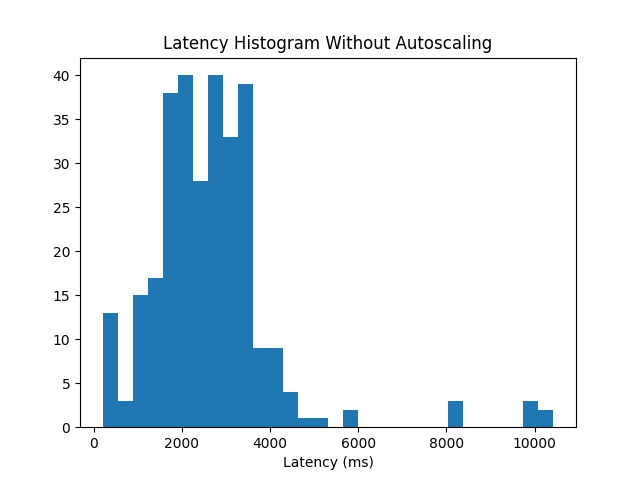
\includegraphics[width=20em]{../plots/latency_without_autoscaling_hist.png}
    \caption{30 iterations, 10 threads}
\end{figure}

\begin{figure}[H]
    \centering
    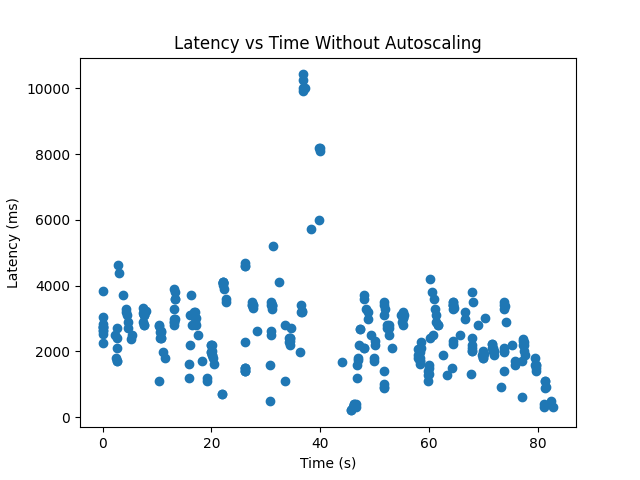
\includegraphics[width=20em]{../plots/latency_without_autoscaling.png}
\end{figure}

\begin{figure}[H]
    \centering
    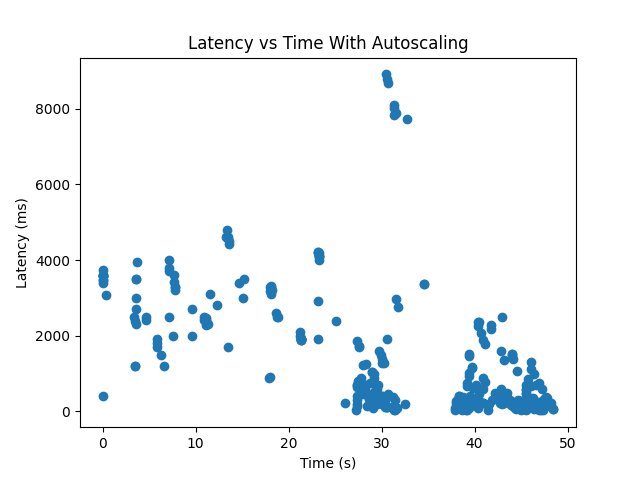
\includegraphics[width=20em]{../plots/latency_with_autoscaling.png}
    \caption{30 iterations, 10 threads}
\end{figure}

\begin{figure}[H]
    \centering
    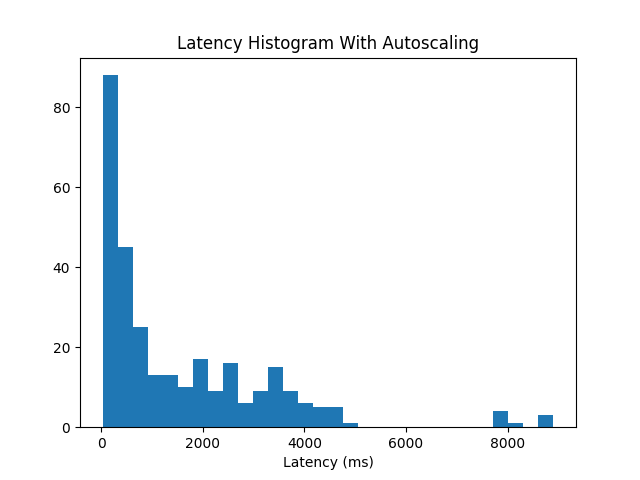
\includegraphics[width=20em]{../plots/latency_with_autoscaling_hist.png}
    \caption{30 iterations, 10 threads}
\end{figure}

\begin{figure}[H]
    \centering
    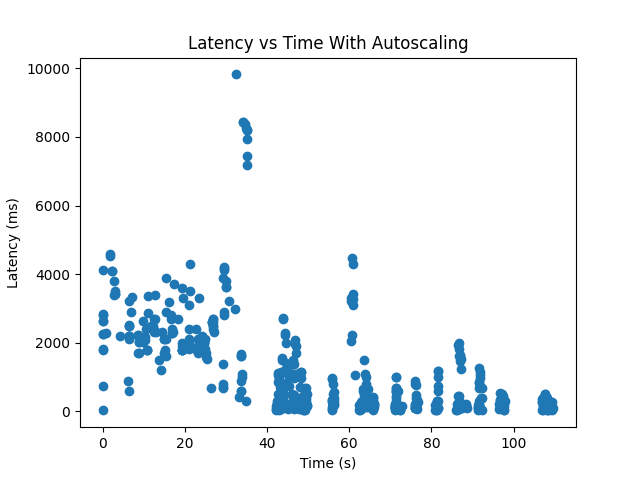
\includegraphics[width=20em]{../plots/latency_with_autoscaling_50.png}
    \caption{50 iterations, 10 threads}
\end{figure}

\begin{figure}[H]
    \centering
    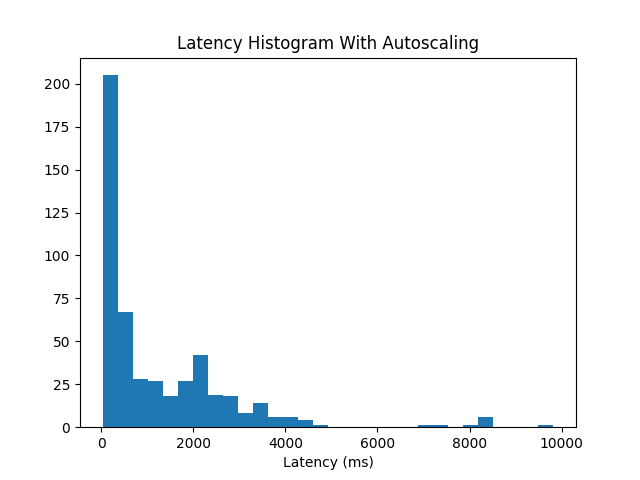
\includegraphics[width=20em]{../plots/latency_with_autoscaling_hist_50.png}
    \caption{50 iterations, 10 threads}
\end{figure}

\begin{figure}[H]
    \centering
    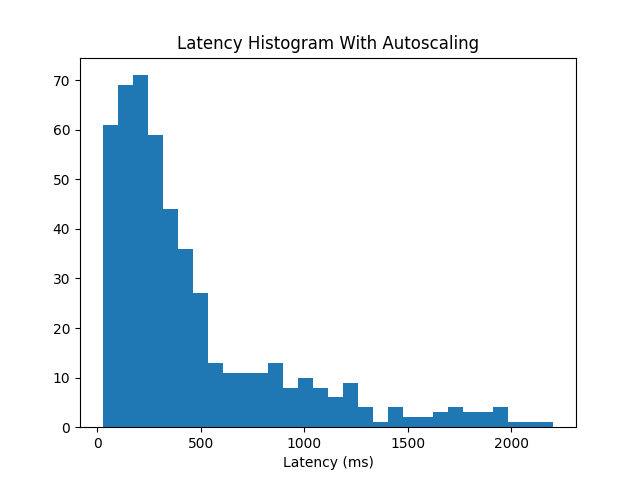
\includegraphics[width=20em]{../plots/latency_with_autoscaling_hist_50_warm.png}
    \caption{50 iterations, 10 threads}
\end{figure}



\end{document}
